\documentclass[oneside]{book}

\usepackage[utf8]{inputenc}
\usepackage[english]{babel}

\usepackage{url}
\usepackage{tikz}
\usetikzlibrary{calc}
\usepackage{float}
\usepackage{ifthen}
\usepackage{siunitx}
\usepackage{lmodern}
\usepackage{amsmath}
\usepackage{listings}
\usepackage{graphicx}
\usepackage{subfiles}
\usepackage{biblatex}
\usepackage{csquotes}
\usepackage{tabularx}
\usepackage{multirow}
\usepackage{geometry}
\usepackage{enumitem}
\usepackage{pdfpages}
\usepackage{bytefield}
\usepackage{microtype}
\usepackage{alphabeta}
\usepackage{xcolor,colortbl}
\usepackage[titletoc]{appendix}
\usepackage[hidelinks]{hyperref}

\providecommand{\main}{.}
\addbibresource{\main/references.bib}   

\usepackage{\main/sty/slashbox}

\newboolean{printBibInSubfiles}
\setboolean{printBibInSubfiles}{true} 
\def\bib{\ifthenelse{\boolean{printBibInSubfiles}}
        {\printbibliography}
        {}
    }

\definecolor{Gray}{gray}{0.85}
\definecolor{LightCyan}{rgb}{0.2,0.7,1}

\newcolumntype{g}{>{\columncolor{Gray}}c}
\newcolumntype{w}{>{\columncolor{white}}c}
\newcolumntype{L}{>{\arraybackslash}X}
\newcolumntype{M}[1]{>{\centering\arraybackslash}m{#1\textwidth}}

\newlist{abbrv}{itemize}{1}
\setlist[abbrv,1]{label=,labelwidth=1in,align=parleft,itemsep=0.1\baselineskip,leftmargin=!}

\DeclareMathOperator*{\argmax}{argmax} 
\DeclareMathOperator*{\argmin}{argmin} 

\graphicspath{{imgs/}}

\geometry{
    left=20mm,
    right=20mm,
    top=20mm,
    bottom=20mm,
    heightrounded
}

\setlength\parindent{0pt}

\begin{document}
\setboolean{printBibInSubfiles}{false}

\subfile{00_misc/cover.tex}
\subfile{00_misc/ack.tex}
\subfile{00_misc/abs.tex}
\subfile{00_misc/fig.tex}
\subfile{00_misc/tab.tex}
\subfile{00_misc/sym.tex}

\subfile{01_intro/introduction.tex}
\subfile{02_theory/ultra_wideband.tex}
\subfile{02_theory/position_estimation.tex}

\subfile{03_firmware/firmware.tex}

\subfile{02_theory/ble_mesh.tex}

\subfile{04_hardware/hardware.tex}
\subfile{05_software/software.tex}
\subfile{06_result/result.tex}

\begin{appendices}
    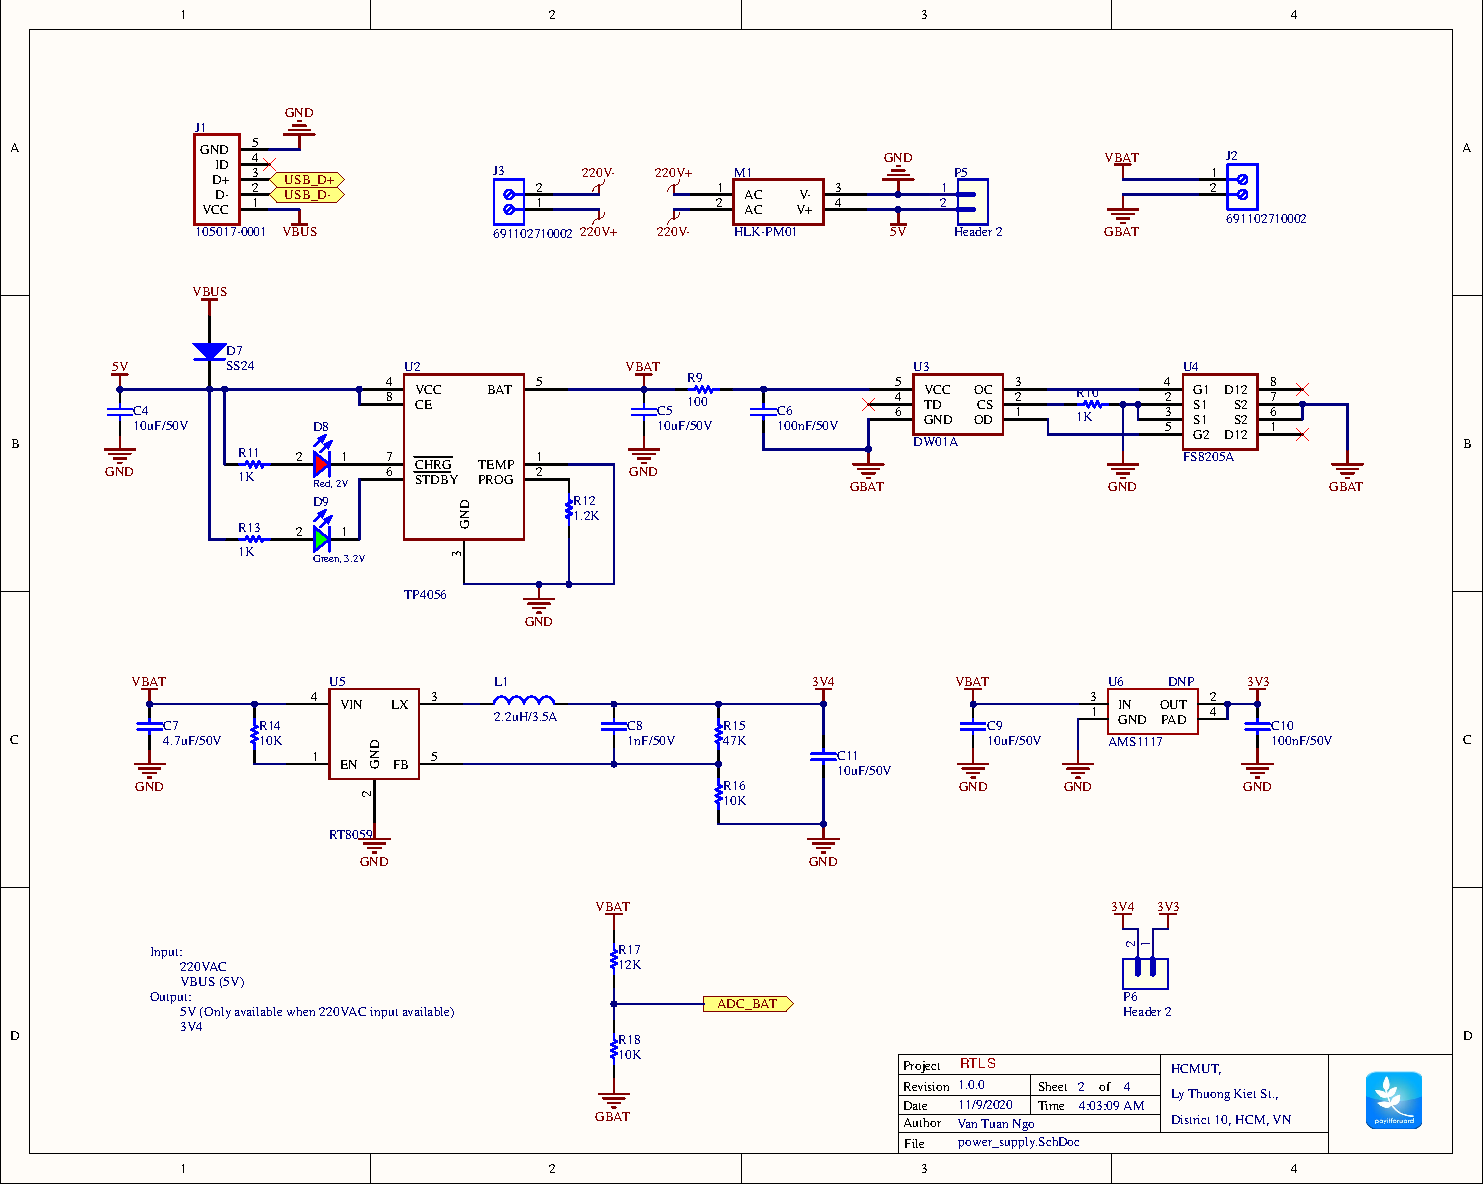
\includepdf[pages=1,pagecommand=\chapter{RTLS Anchor Board (Altium Designer)},width=\textwidth, offset=0 -1cm]{RTLS-2020-11-09--04-03.PDF}
    \includepdf[pages=2-,pagecommand={},width=\textwidth]{RTLS-2020-11-09--04-03.PDF}
\end{appendices}

\begin{appendices}
    \chapter{RTLS Anchor House (SolidWorks)}
    \begin{figure}[H]
        \begin{center}
            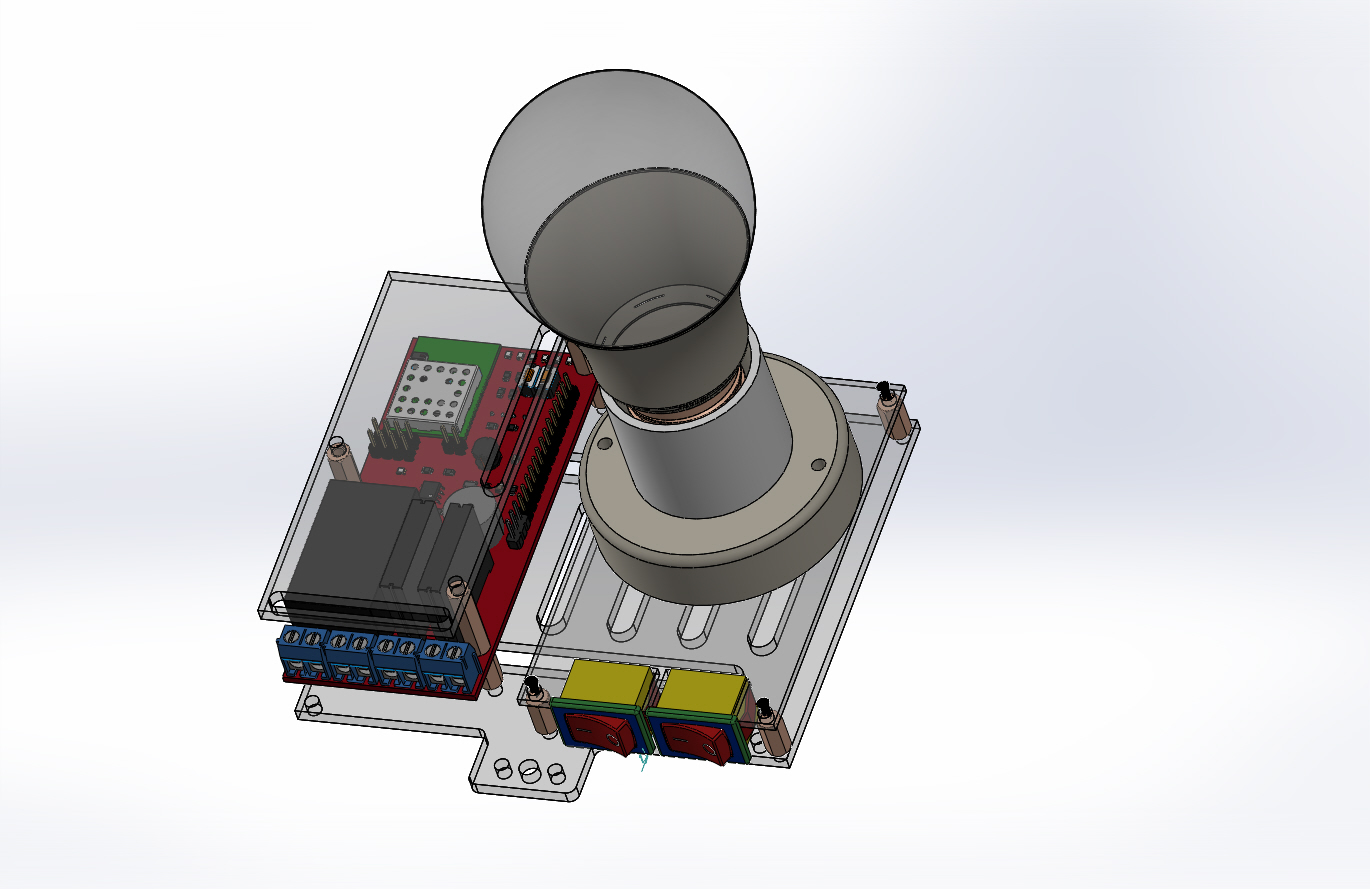
\includegraphics[scale=0.4]{Assem.JPG}
        \end{center}
        \caption{RTLS SolidWorks Design}
        \label{fig:RTLS_SolidWork_Design}
    \end{figure}
\end{appendices}

\printbibliography[heading=bibintoc,title={References}]

\end{document}
